\documentclass[a4paper, 12pt]{article}
\usepackage{graphicx}
\usepackage[czech]{babel}
\usepackage[utf8]{inputenc}
\usepackage[T1]{fontenc}
\usepackage{amsmath}
\usepackage{amssymb}
\usepackage{pdfpages}
\usepackage{mathrsfs}
\usepackage{siunitx}
\usepackage{xcolor}
\usepackage{titlesec}
\usepackage{wrapfig}

\setcounter{secnumdepth}{4}

\titleformat{\paragraph}
{\normalfont\normalsize\bfseries}{\theparagraph}{1em}{}
\titlespacing*{\paragraph}
{0pt}{3.25ex plus 1ex minus .2ex}{1.5ex plus .2ex}

\sisetup{%
     output-decimal-marker = {.},
     inter-unit-product = \ensuremath{{}\cdot{}}
        }
        
\author{A18B0474P - Jiří Švamberg}
\title{Projekt 5}
\date{\today}

\setlength{\hoffset}{-1.8cm} 
\setlength{\voffset}{-2cm}
\setlength{\textheight}{24.0cm} 
\setlength{\textwidth}{17cm}

\begin{document}
	\begin{titlepage}
		\maketitle
		\begin{figure}
			\centering
			
\includegraphics{Obrazky/FAV-logo.pdf}
			
\includegraphics{Obrazky/zcu-logo.pdf}
			
\includegraphics[scale=0.3]{Obrazky/KKY_logo_cz.pdf}
		\end{figure}
		\thispagestyle{empty}
		\newpage
	\end{titlepage}

	\tableofcontents
	\newpage
	\section{Zadání}
		\begin{enumerate}
			\item Navrhněte zjednodušený model soustavy kvadrotorová helikoptéra - břemeno\\
			\item Pro zjednodušený model navrhněte regulátor\\
			\item Implementujte regulátor do zjednodušeného modelu\\
		\end{enumerate}
		\clearpage
	\section{Zjednodušený model}
		\subsection{Návrh zjednodušeného modelu}		
			Zjednodušený model budeme navrhovat ve 2D jako kyvadlo zavěšené na vozíku.
			\begin{wrapfigure}{r}{0pt}
				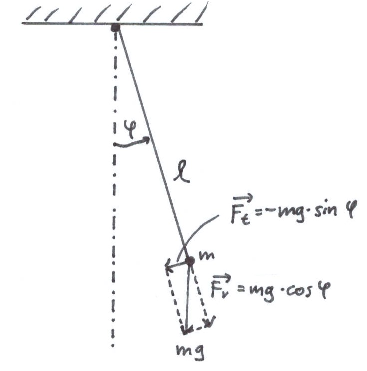
\includegraphics[scale=0.75]{Obrazky/Kyvadlo.pdf}
				\caption{Schéma jednoduchého kyvadla}
				\label{schema kyvadla}
			%\end{wrapfigure}
			%\begin{wrapfigure}{r}{0pt}
				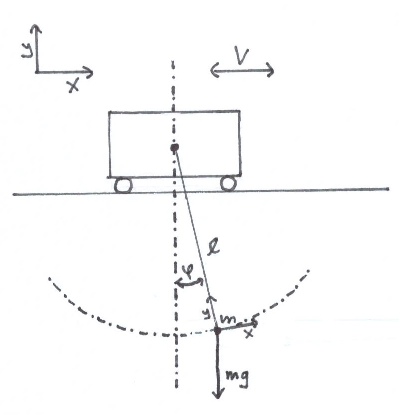
\includegraphics[scale=0.75]{Obrazky/Vozik-kyvadlo.pdf}
				\caption{Schéma soustavy vozík-kyvadlo}
				\label{schema vozik-kyvadlo}
			\end{wrapfigure}
			Pro potřeby návrhu tohoto modelu budeme uvažovat lano závěsu jako dokonale nepružné, o stálé délce $l$ a nulové hmotnosti $m_l = \SI{0}{\kilogram}$. Úhel vychýlení závěsu od osy vozíku označíme jako $\varphi$. Jako těleso si představíme bezrozměrný hmotný bod o hmotnosti $m$.\\
			Pro jednoduché kyvadlo připevněné k nepohybujícímu se tělesu o kinetické energii $T = \frac{1}{2}mv^2$ a potenciální energii $V = -mgl\cos\varphi$ (obr. \ref{schema kyvadla}) platí pohybová rovnice:
			\begin{align*}
				\ddot{\varphi}+\frac{g}{l}\sin\varphi=0
			\end{align*}
			Po zavěšení jednoduchého kyvadla na vozík(obr. \ref{schema vozik-kyvadlo}) budeme muset ještě do modelu přidat dynamiku vozíku o hmotnosti $M$. Na ten může působit síla ve směru osy x. Pro hmotný bod, zavěšený na laně budeme muset spočítat souřadnice $\left[u, v\right]$, jelikož při pohybu vozíku se nepohybuje po jasné trajektorii (kružnice, přímka):
			\begin{align*}
				u &= x + l\sin\varphi \rightarrow \dot{u} = \dot{x}+l\dot{\varphi}\cos\varphi\\
				v &= l\cos\varphi \rightarrow \dot{v} = -l\dot{\varphi}\sin\varphi
			\end{align*} 
			K odvození modelu využijeme Lagrangeovu metodu.\\
			Potenciální energii $V$ budeme uvažovat stejnou, jako u jednoduchého kyvadla.
			\begin{align*}
				V = -mgl\cos{\varphi}
			\end{align*}
			Jako základ pro vzorec kinetické energie použijeme vzorec kinetické energie obyčejného matematického kyvadla $T = \frac{1}{2}mv^2$. Musíme ale uvažovat rychlost ve směru všech souřadnic ($x$, $u$, $v$).
			\begin{align*}
				T &= \frac{1}{2}M\dot{x}^2+\frac{1}{2}m\dot{u}^2+\frac{1}{2}m\dot{v}^2
			\end{align*}
			Po dosazení souřadnic pro hmotný bod zavěšený na laně dostaneme kinetickou energii ve tvaru:
			\begin{align*}
				T &= \frac{1}{2}M\dot{x}^2+\frac{1}{2}m\left(\dot{x}+l\dot{\varphi}\cos\varphi\right)^2+\frac{1}{2}m\left(-l\dot{\varphi}\sin\varphi\right)^2
			\end{align*}
			Zjistíme si Lagrangián $L = T - V$:
			\begin{align*}
				L = \frac{1}{2}M\dot{x}+\frac{1}{2}m\left(\dot{x}+l\dot{\varphi}\cos\varphi\right)^2+\frac{1}{2}m\left(l\dot{\varphi}\sin\varphi\right)^2+mgl\cos\varphi
			\end{align*}
			, který nyní budeme parciálně derivovat.
			\begin{align*}
				\frac{\partial L}{\partial\dot{x}} &= M\dot{x}+m\dot{x}+ml\dot{\varphi}\cos\varphi\\
				\frac{\partial L}{\partial x} &= 0\\
				\frac{\partial L}{\partial \dot{\varphi}} &= m\dot{x}l\cos\varphi - ml^2\dot{\varphi}\\
				\frac{\partial L}{\partial \varphi} &= -m\dot{x}l\dot{\varphi}\sin\varphi-l^2\dot{\varphi}^2\cos\varphi\sin\varphi+ml^2\dot{\varphi}^2\sin\varphi\cos\varphi-mgl\sin\varphi
			\end{align*}
			Vztahy pro hledané dvě rovnice vypadají následovně:
			\begin{align*}
				\frac{\mathrm{d}}{\mathrm{d}t}\left(\frac{\partial L}{\partial \dot{x}}\right)-\frac{\partial L}{\partial x} = f\\
				\frac{\mathrm{d}}{\mathrm{d}t}\left(\frac{\partial L}{\partial \dot{\varphi}}\right)-\frac{\partial L}{\partial \varphi} = 0
			\end{align*}
			, kde f je síla působící na vozík. Nyní můžeme dopočítat dvě rovnice modelu vozík-kyvadlo.
			\begin{align}
				\left(M+m\right)\ddot{x}+ml\ddot{\varphi}\cos\varphi-ml\dot{\varphi}^2\sin\varphi = f
				\label{rovnice_model_1}\\
				\ddot{x}\cos\varphi+g\sin\varphi-l\ddot{\varphi} = 0
			    \label{rovnice_model_2}
			\end{align}
		\subsection{Linearizace modelu}
			Aby bylo s modelem snazší pracovat, linearizujeme ho v okolí pracovního bodu, tzn. $\varphi = 0$. Díky tomu můžeme uvažovat:
			\begin{align*}
				\sin\varphi &\approx \varphi\\
				\cos\varphi	&\approx 1
			\end{align*}
			Po dosazení do rovnic \ref{rovnice_model_1} a \ref{rovnice_model_2} dostaneme nové jednodušší rovnice \ref{rovnice_model_lin_1} a \ref{rovnice_model_lin_2}.
			\begin{align}
				\left(M+m\right)\ddot{x}+ml\ddot{\varphi}-ml\dot{\varphi}^2\varphi = f
				\label{rovnice_model_lin_1}\\
				\ddot{x}+g\varphi-l\ddot{\varphi} = 0
			    \label{rovnice_model_lin_2}
			\end{align}
			Dále můžeme vyjádřit nejvyšší derivace:
			\begin{align*}
				f_1: \ddot{x}&=\frac{-ml\ddot{\varphi}+ml\dot{\varphi}^2\varphi+f}{m+M}\\
				f_2: \ddot{\varphi}&=\frac{\ddot{x}+g\varphi}{l}
			\end{align*}
			Vidíme, že rovnice na sobě závisí. Můžeme tedy jednu dosadit do druhé a opačně.
			\begin{align*}
				\ddot{x}&=\frac{-mg\varphi+ml\dot{\varphi}^2\varphi+f}{2m+M}\\
				\ddot{\varphi}&=\frac{ml\dot{\varphi}^2\varphi+f+mg\varphi+Mg\varphi}{l\left(2m+M\right)}
			\end{align*}
		\subsection{Stavový popis systému}
			Stavový popis systému uvažujeme ve tvaru:
			\begin{align*}
				\dot{x} &= \mathbf{A}\vec{x}+\mathbf{B}\vec{u}\\
				y &= \mathbf{C}\vec{x}   %+\mathbf{D}\vec{u}
			\end{align*}
			, kde 
			\begin{align*}
				\mathbf{A} &= \left[\begin{matrix}
					0 & 0 & 1 & 0\\
					0 & 0 & 0 & 1\\
					\frac{\partial f_1}{\partial \dot{x}} & \frac{\partial f_1}{\partial \dot{\varphi}} & \frac{\partial f_1}{\partial x} & \frac{\partial f_1}{\partial\varphi}\\
					\frac{\partial f_2}{\partial \dot{x}} & \frac{\partial f_2}{\partial \dot{\varphi}} & \frac{\partial f_2}{\partial x} & \frac{\partial f_2}{\partial \varphi}	
				\end{matrix}\right]\\
				\mathbf{B} &= \left[\begin{matrix}
					0\\
					0\\
					\frac{\partial f_1}{\partial f}\\
					\frac{\partial f_2}{\partial f}
				\end{matrix}\right]\\
				\mathbf{C} &= \left[\begin{matrix}
					1 & 0 & 0 & 0\\
					0 & 1 & 0 & 0\\
					0 & 0 & 1 & 0\\
					0 & 0 & 0 & 1
				\end{matrix}\right]
			\end{align*}
			Zavedeme si stavové proměnné
			\begin{align*}
				x_1 = \dot{x}\\
				x_2 = \dot{\varphi}\\
				x_3 = x\\
				x_4 = \varphi\\
				u = f
			\end{align*}
			Dosadíme do rovnic a budeme moct derivovat.
			\begin{align*}
				f_1: \ddot{x}&=\frac{l m x_4 x_2^2 + u - g m x_4}{M + 2m}\\
				f_2: \ddot{\varphi}&=\frac{l m x_4 x_2^2 + u + M g x_4 + m g x_4}{l\left(M+2m\right)}
			\end{align*}
			Po zderivování dostaneme matice:
			\begin{align*}
				\mathbf{A} &= \left[\begin{matrix}
					0 & 0 & 1 & 0\\
					0 & 0 & 0 & 1\\
					0 & \frac{2lmx_4x_2}{M+2m} & 0 & \frac{lmx_2^2-gm}{M+2m}\\
					0 & \frac{2lmx_4x_2}{l\left(M+2m\right)} & 0 & \frac{lmx_2^2+Mg+mg}{l\left(M+2m\right)}
				\end{matrix}\right]\\
				\mathbf{B} &= \left[\begin{matrix}
					0\\
					0\\
					\frac{1}{M+2m}\\
					\frac{1}{l\left(M+2m\right)}
				\end{matrix}\right]\\
				\mathbf{C} &= \left[\begin{matrix}
					1 & 0 & 0 & 0\\
					0 & 1 & 0 & 0\\
					0 & 0 & 1 & 0\\
					0 & 0 & 0 & 1
				\end{matrix}\right]
			\end{align*}
			, celý popis bude tedy ve tvaru
			\begin{align*}
				\dot{x} &= \left[\begin{matrix}
					0 & 0 & 1 & 0\\
					0 & 0 & 0 & 1\\
					0 & \frac{2lmx_4x_2}{M+2m} & 0 & \frac{lmx_2^2-gm}{M+2m}\\
					0 & \frac{2lmx_4x_2}{l\left(M+2m\right)} & 0 & \frac{lmx_2^2+Mg+mg}{l\left(M+2m\right)}
				\end{matrix}\right]
				\left[\begin{matrix}
					x_1\\
					x_2\\
					x_3\\
					x_4
				\end{matrix}\right]+
				\left[\begin{matrix}
					0\\
					0\\
					\frac{1}{M+2m}\\
					\frac{1}{l\left(M+2m\right)}
				\end{matrix}\right]u\\
				y &= \left[\begin{matrix}
					1 & 0 & 0 & 0\\
					0 & 1 & 0 & 0\\
					0 & 0 & 1 & 0\\
					0 & 0 & 0 & 1
				\end{matrix}\right]x
			\end{align*}
\end{document}